\section{Own approach}\label{sec:approach}\par
Our approach is based on several steps, as shown in Figure \ref{fig:our_approach}. First of all, we looked for possible sources that might be relevant for the preparation of our paper. 
On the basis of primarily scientific literature, we acquired the necessary theoretical basics that we needed to work on the topic, while carefully considering also critical sources.
In addition to the six conference papers on the topic given to us, we also considered other, more recent conference- and whitepapers to work on the topic.
Based on the given papers and other selected papers, we created a Mindmap to determine possible visions and challenges and their correlations in the context of industrial edge computing. At the same time we created a high-level timeline for working on this paper.
Based on our Mindmap we discussed possible visions and challenges. In addition to the aspects from the papers given to us, we also considered aspects from more recent conference- and whitepapers.\par
During our research we also noticed that the boundaries between Edge Computing and Fog Computing are increasingly disappearing and that both paradigms are more and more seen in interaction with each other.
Therefore, the focus of this paper is not only on visions and challenges related to industrial Edge Computing, but also on aspects related to Fog Computing.

\begin{figure}[h]
    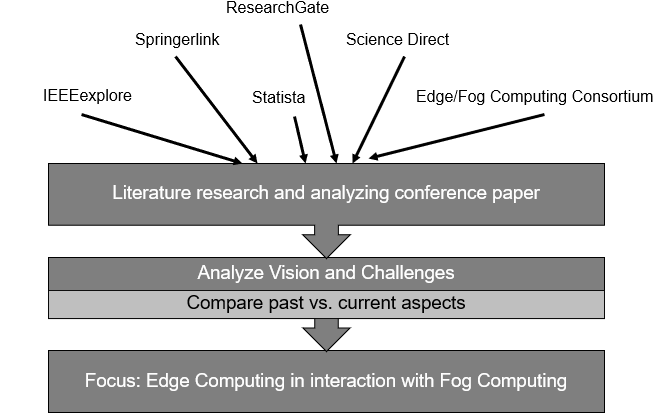
\includegraphics[width=1\textwidth,height=0.65\textwidth]{resources/images/our_approach.png}
    \caption{Own approach: Based on analyzing multiple conference- and whitepaper}
    \label{fig:our_approach}
\end{figure}

In the following chapter, selected visions and challenges are identified and explained in detail.